\documentclass[11pt,a4paper]{article}

\usepackage{amsmath,amssymb}
\usepackage{graphicx}
\usepackage{booktabs}
\usepackage{natbib}
\usepackage[margin=1in]{geometry}
\usepackage{enumitem}
\usepackage{hyperref}
\usepackage{xcolor}

\hypersetup{
  colorlinks=true,
  linkcolor=blue!50!black,
  citecolor=blue!50!black,
  urlcolor=blue!60!black
}

\graphicspath{{figures/}}

\title{Anisotropic Hubble expansion from an off-center observer\\
in a Sedov--Taylor blast-wave universe}
\author{C.\ A.}
\date{2026-09-19}

\begin{document}
\maketitle

\begin{abstract}
We synthesize a Newtonian working model in which the Universe expands as a
Sedov--Taylor (ST) homologous blast about a \emph{real} geometric center of
expansion (CoE) beyond the observable horizon, with the observer off-center.
Homology alone yields an isotropic apparent Hubble parameter; anisotropy
requires a homology-breaking mechanism. We take that mechanism to be Gauss /
shell-theorem gravity from a centrally concentrated, radially decreasing
density $\rho(r)$, so $g=-GM(<r)/r^2$ (not a uniform ball). Preferring
time-integrated peculiar velocities over a bolt-on impulse $u\sim\alpha g/H$,
ideal integration only rescales the amplitude
($\alpha\to\alpha_{\mathrm{eff}}$) and does \emph{not} flip the angular shape
of the Migkas-style normalization $A(\varphi)$; expand versus collapse does.
Mapping $A_{\mathrm{hratio}}\propto H_{\mathrm{obs}}/H$ against the Migkas
et~al.\ (2020) $A$ versus Galactic longitude pattern, first-principles
ST+Gauss geometry alone reaches $R^2\approx0.543$. A diagnostic
Amp$\times\sin$ phase rotation raises $R^2\approx0.746$; a multiplicative
$2\ell$ residual layer reaches $R^2\approx0.875$ (RMSE $0.038\to0.029$).
Amp$\times\sin$ and the $2\ell$ multiplier are phenomenological; the
first-principles claim is the geometry. The CMB remains the principal
adversary (spherical off-center voids are dipole-limited to
$\sim15\,\mathrm{Mpc}$). This paper does not claim to have falsified the
cosmological principle.
\end{abstract}

\tableofcontents
\newpage

%----------------------------------------------------------------------
\section{Introduction}
\label{sec:intro}

The cosmological principle (CP) asserts statistical homogeneity and isotropy on
large scales: no preferred center, and a suitably defined Hubble expansion that
is isotropic about every comoving observer. Late-time directional probes contest
that claim at the several-to-tens-of-percent level. In particular, Migkas
et~al.~\citep{Migkas2020} reported that the normalization $A$ of the X-ray
cluster $L_X$--$T$ relation varies with Galactic longitude (their Fig.~6), with
a preferred direction near $(\ell,b)\sim(280^\circ,-20^\circ)$ and a maximum
luminosity-distance variation of order $\sim16\pm3\%$ under an isotropic-scaling
interpretation. Those results remain contested---bulk flows, absorption,
calibration, and scatter can all mimic directional signals---but they supply the
empirical sky pattern against which any centered alternative must be aimed.

The program synthesized here is stronger than a mild $\Lambda$CDM tweak. It
asserts:
\begin{enumerate}[leftmargin=*,itemsep=2pt]
\item The Universe has a \textbf{real center of expansion (CoE)}.
\item That CoE lies \textbf{beyond the observable horizon}.
\item We are an \textbf{off-center observer} at Euclidean (Newtonian) distance
  $D$ from the CoE.
\item Expansion is usefully modeled, at the Newtonian skeleton level, by a
  \textbf{Sedov--Taylor blast} with a \textbf{radially decreasing} density
  $\rho(r)$ about the CoE; gravity follows Gauss's law with enclosed mass
  $M(<r)$ identified with the mass between us and the CoE.
\end{enumerate}
The scientific goal is to locate that center---or kill the idea if CMB isotropy
and related probes make a real center untenable~\citep{Alnes2006,Kodama2010,Saadeh2016,Planck2018VII}.

Historical cousins include Fennelly's off-center Hubble anisotropy~\citep{Fennelly1977},
Bertschinger's cosmological ST shocks~\citep{Bertschinger1983}, Smoller--Temple
shock cosmologies inside / beyond a Hubble-scale black hole~\citep{SmollerTemple1998,SmollerTemple2002},
and the LTB off-center CMB literature~\citep{Alnes2006,Kodama2010,Blomqvist2010}.
None combines ST+Gauss geometry, a beyond-horizon CoE, and a Migkas $A(\ell)$
target with explicit CMB accounting; that gap is the present niche.

%----------------------------------------------------------------------
\section{Model: Sedov--Taylor background, Gauss gravity, off-center observer}
\label{sec:model}

\subsection{Geometry}
\label{sec:geom}

Place the CoE at the origin. The observer sits at $\vec{D}$ with $D=\|\vec{D}\|$.
A source is at $\vec{r}$ (CoE-radius $r=\|\vec{r}\|$), with observer--source
separation $\vec{d}=\vec{r}-\vec{D}$, $d=\|\vec{d}\|$, and line of sight
$\hat{n}=\vec{d}/d$. The preferred axis $\hat{D}=\vec{D}/D$ points from CoE to
observer; the direction from observer toward the CoE is $-\hat{D}$.

Toy calculations place sources on an observer-centered circle of fixed $d$ with
Earth-centric angle $\varphi$ measured from $+\hat{D}$ (anti-center):
\begin{equation}
\hat{n}=(\cos\varphi,\sin\varphi),\qquad \mu\equiv\hat{n}\cdot\hat{D}=\cos\varphi.
\end{equation}
Thus $\varphi=0$ looks away from the CoE and $\varphi=\pi$ looks toward it.
When comparing to Galactic longitude $\ell$, an overall sky-axis orientation is
absorbed into a phase (Sec.~\ref{sec:fits}). Scale lengths entering the mass
profile are denoted $L$ (or $r_s$); the dimensionless ratios of interest are
$d/D$, $D/L$, and $M/M_0$ (mass in units of a reference $M_0$).

\begin{figure}[t]
\centering
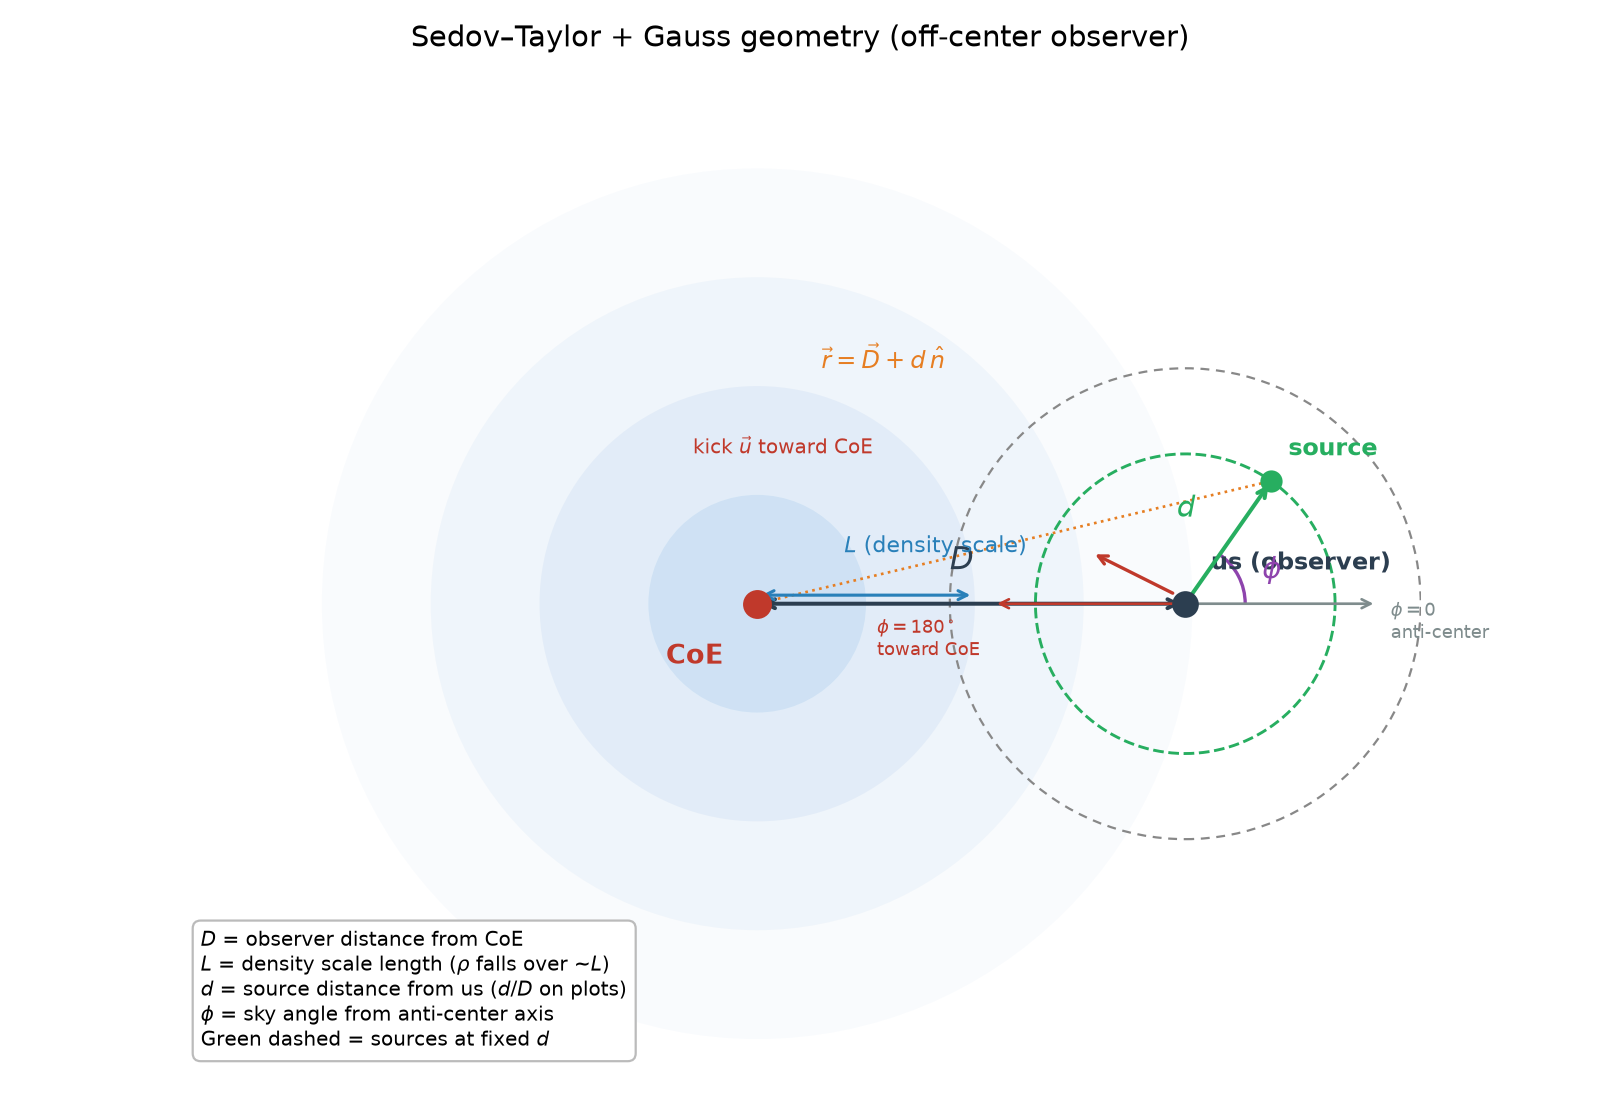
\includegraphics[width=0.72\textwidth]{geometry_CoE_observer.png}
\caption{Geometry of an off-center observer at distance $D$ from a real CoE,
with source distance $d$ and angle $\varphi$ from the preferred axis.
First-principles ST+Gauss kinematics are computed in this plane (then rotated
on the sky as a diagnostic).}
\label{fig:geom}
\end{figure}

\subsection{Homologous Sedov--Taylor background}
\label{sec:st}

Classical Sedov--Taylor blast front in ambient density $\rho_0$ with energy $E$:
\begin{equation}
R_{\mathrm{ST}}(t)=\xi\Bigl(\frac{E}{\rho_0}\Bigr)^{1/5}t^{2/5},\qquad
H(t)\equiv\frac{\dot{R}_{\mathrm{ST}}}{R_{\mathrm{ST}}}=\frac{2}{5t}.
\label{eq:ST}
\end{equation}
Interior working assumption (homologous expansion or collapse):
\begin{equation}
\vec{v}(\vec{r},t)=H_{\mathrm{bg}}\,\vec{r},\qquad
H_{\mathrm{bg}}=+H\quad\text{(expand)}\quad\text{or}\quad -H\quad\text{(collapse)}.
\label{eq:homologous}
\end{equation}
Observer and source velocities in the CoE frame are then
$\vec{v}_O=H_{\mathrm{bg}}\vec{D}$ and $\vec{v}_S=H_{\mathrm{bg}}\vec{r}$, so
\begin{equation}
\vec{v}_{\mathrm{rel}}=H_{\mathrm{bg}}\,\vec{d},\qquad
v_{\mathrm{los}}=\vec{v}_{\mathrm{rel}}\cdot\hat{n}=H_{\mathrm{bg}}\,d,\qquad
H_{\mathrm{obs}}=\frac{v_{\mathrm{los}}}{d}=H_{\mathrm{bg}}.
\label{eq:pureST}
\end{equation}
\textbf{Critical kinematic result:} pure homology yields
$H_{\mathrm{obs}}=H_{\mathrm{bg}}$ \emph{independent of direction}, for any
offset $D$. Geometry alone does not produce Migkas-like anisotropy. Anisotropy
requires breaking homology (gravity, non-homologous ST structure, or
relativistic / light-cone effects). Cosmological identification of
$(E,\rho_0,\xi)$ remains undefined; Eq.~\eqref{eq:ST} is a similarity scaffold,
not a derivation of FLRW~\citep{Bertschinger1983}.

\subsection{Gauss gravity with decreasing density}
\label{sec:gauss}

Under spherical symmetry, Newton's shell theorem / Gauss's law gives
\begin{equation}
\vec{g}(\vec{r})=-\frac{G\,M(<r)}{r^2}\,\hat{r},\qquad
M(<r)=\int_0^r 4\pi s^2\rho(s)\,ds.
\label{eq:gauss}
\end{equation}
The working density is \textbf{centrally concentrated and radially decreasing}.
A convenient Phase~A profile (incomplete-gamma cumulative of
$\rho\propto e^{-r/L}$) is
\begin{equation}
\frac{M(<r)}{M}=1-e^{-X}\Bigl(1+X+\frac{X^2}{2}\Bigr),\qquad X=\frac{r}{L}.
\label{eq:profile}
\end{equation}
\textbf{Rejected special case:} uniform ball $\rho=\mathrm{const}\Rightarrow
M(<r)\propto r^3\Rightarrow g\propto -r$, which produces only a monopole shift
in $H_{\mathrm{obs}}$ and no sky anisotropy. Decreasing $\rho$ makes $M(<r)$
grow slower than $r^3$, retaining tidal $1/r^2$ structure near $r\sim D$.

Chris identifies the relevant enclosure with the mass toward the CoE. At
observer scale the dimensionless strength is
\begin{equation}
\kappa\equiv\frac{G\,M(<D)}{D^3 H^2}.
\label{eq:kappa}
\end{equation}
For an $\Omega_m\sim0.3$ critical sphere one has the natural scale
$\kappa_{\mathrm{natural}}\sim\Omega_m/2\sim0.15$; the program's working
$\kappa\sim\mathcal{O}(0.1$--$1)$ relative to $M_{\mathrm{crit}}(<D)$ is meant
to be natural, not absurd.

%----------------------------------------------------------------------
\section{Bolt-on peculiar velocity versus ideal time-integrated gravity}
\label{sec:boltideal}

\subsection{Bolt-on impulse}
Acceleration is not velocity. A common order-of-magnitude ansatz is an impulse
over a Hubble time,
\begin{equation}
\vec{u}(\vec{r})=-\alpha\,\frac{G\,M(<r)}{r^2 H}\,\hat{r},\qquad
\alpha\sim\mathcal{O}(1),
\label{eq:bolton}
\end{equation}
with relative peculiar contribution
\begin{equation}
\delta v=\bigl[\vec{u}(\vec{r})-\vec{u}(\vec{D})\bigr]\cdot\hat{n},\qquad
H_{\mathrm{obs}}=H_{\mathrm{bg}}+\frac{\delta v}{d}.
\label{eq:Hobs}
\end{equation}
On an observer-centered circle of radius $d=\varepsilon D$ (code units often
take $\varepsilon\sim\mathrm{few}\times10^{-1}$), Eq.~\eqref{eq:Hobs} is the
closed form used throughout the project's forward maps
(\texttt{H\_obs\_circle}).

\subsection{Ideal time integration}
Preferring physics from the blast start, one integrates $g$ along homologous
trajectories. Three Newtonian treatments yield effective bolt-on amplitudes
$\alpha_{\mathrm{eff}}$~\citep[cf.\ project notes]{Bertschinger1983}:
\begin{enumerate}[leftmargin=*,itemsep=2pt]
\item \textbf{Frozen path:} $\Delta v=\int_{t_i}^{t_f}g(r_{\mathrm{bg}}(t))\,dt$
  $\Rightarrow$ $\alpha_{\mathrm{eff}}=2\bigl(1-\eta^{1/5}\bigr)$ with
  $\eta=t_i/t_f$ (approaches $2$ as $\eta\to0$).
\item \textbf{Hubble drag:} $\mathrm{d}u/\mathrm{d}t+Hu=g$ $\Rightarrow$
  $\alpha_{\mathrm{eff}}=(2/3)\bigl(1-\eta^{3/5}\bigr)$ (approaches $2/3$).
\item \textbf{Nonlinear ODE:} $\ddot{r}=-(6/25)r/t^2-GM/r^2$ (ST background
  acceleration plus gravity).
\end{enumerate}
\textbf{Key structural result:} time integration only rescales amplitude
($\alpha\to\alpha_{\mathrm{eff}}$). It does \emph{not} invent a new small-$\kappa$
regime, and it does \emph{not} flip the angular form of $A(\varphi)$. Only the
sign of the background expansion---expand ($+H$) versus collapse ($-H$)---flips
the trough/peak morphology after the nonlinear $A$ map (Fig.~\ref{fig:expand}).

\begin{figure}[t]
\centering
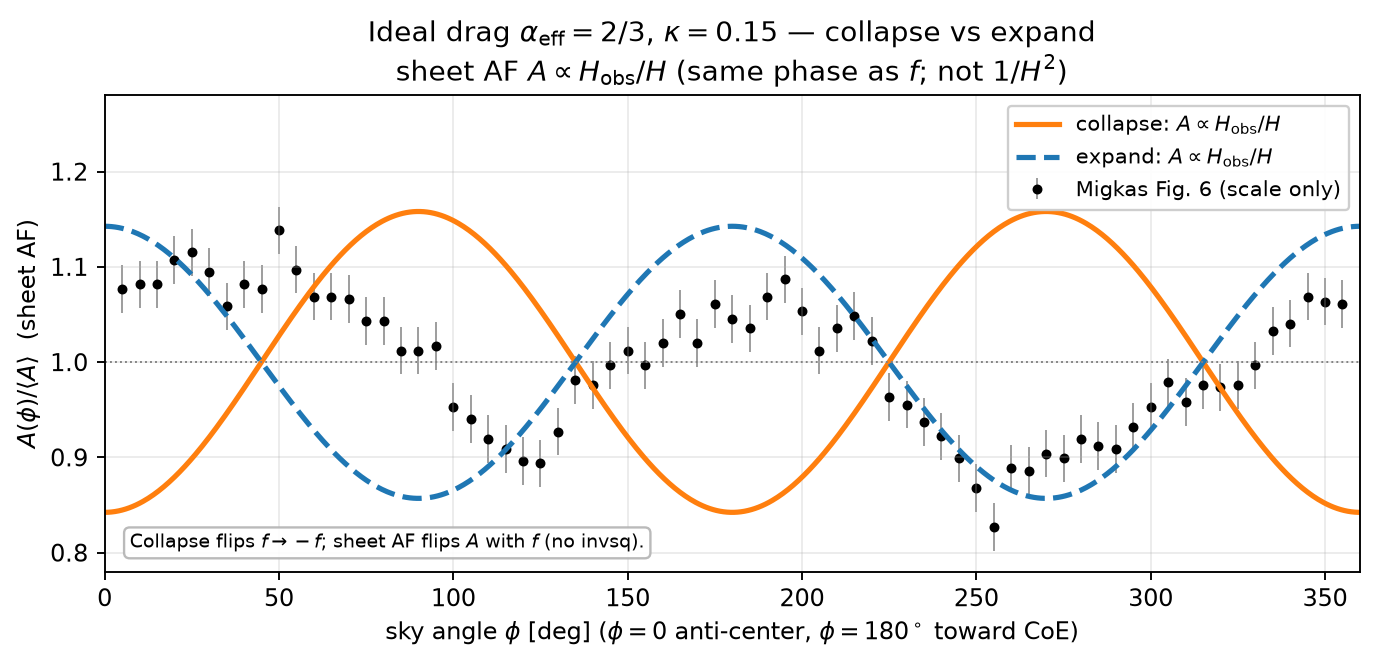
\includegraphics[width=0.85\textwidth]{A_vs_angle_ideal_collapse.png}
\caption{Collapse versus expand under ideal Hubble drag, mapped with sheet AF
$A\propto H_{\mathrm{obs}}/H$ (mean-renormalized; Migkas points for scale only).
Opposite $H_{\mathrm{bg}}$ flips the trough/peak morphology; there is no
$1/H^2$ inversion here. Ideal integration only rescales amplitude.
No Amp$\times\sin$ / $2\ell$ layers.}
\label{fig:expand}
\end{figure}

%----------------------------------------------------------------------
\section{From $H_{\mathrm{obs}}$ to $A(\varphi)$ and Migkas Fig.~6}
\label{sec:Amap}

Migkas et~al.~\citep{Migkas2020} map the $L_X$--$T$ normalization $A$ in
$\Delta\ell=90^\circ$ Galactic-longitude strips. Under isotropic-scaling
assumptions, $A$ tracks luminosity distance (hence inverse powers of an
effective $H$). Two mean-renormalized proxies are used in this program:
\begin{align}
A_{\mathrm{hratio}}&\propto\frac{H_{\mathrm{obs}}}{H}
  \qquad\text{(primary; Chris sheet ``AF'')},
  \label{eq:Ahratio}\\
A_{\mathrm{invsq}}&\propto\frac{1}{(H_{\mathrm{obs}}/H)^2}
  \qquad\text{($L_X$--$T$ / $D_L$-motivated alternative)}.
  \label{eq:Ainvsq}
\end{align}
Both are then optionally smoothed with a wrap-around $\Delta\ell=90^\circ$
boxcar to match Migkas's strip geometry. Empirically,
$A_{\mathrm{invsq}}$ \emph{inverts} troughs and peaks relative to
$A_{\mathrm{hratio}}$; sheet comparisons therefore prefer
Eq.~\eqref{eq:Ahratio}.

\begin{figure}[t]
\centering
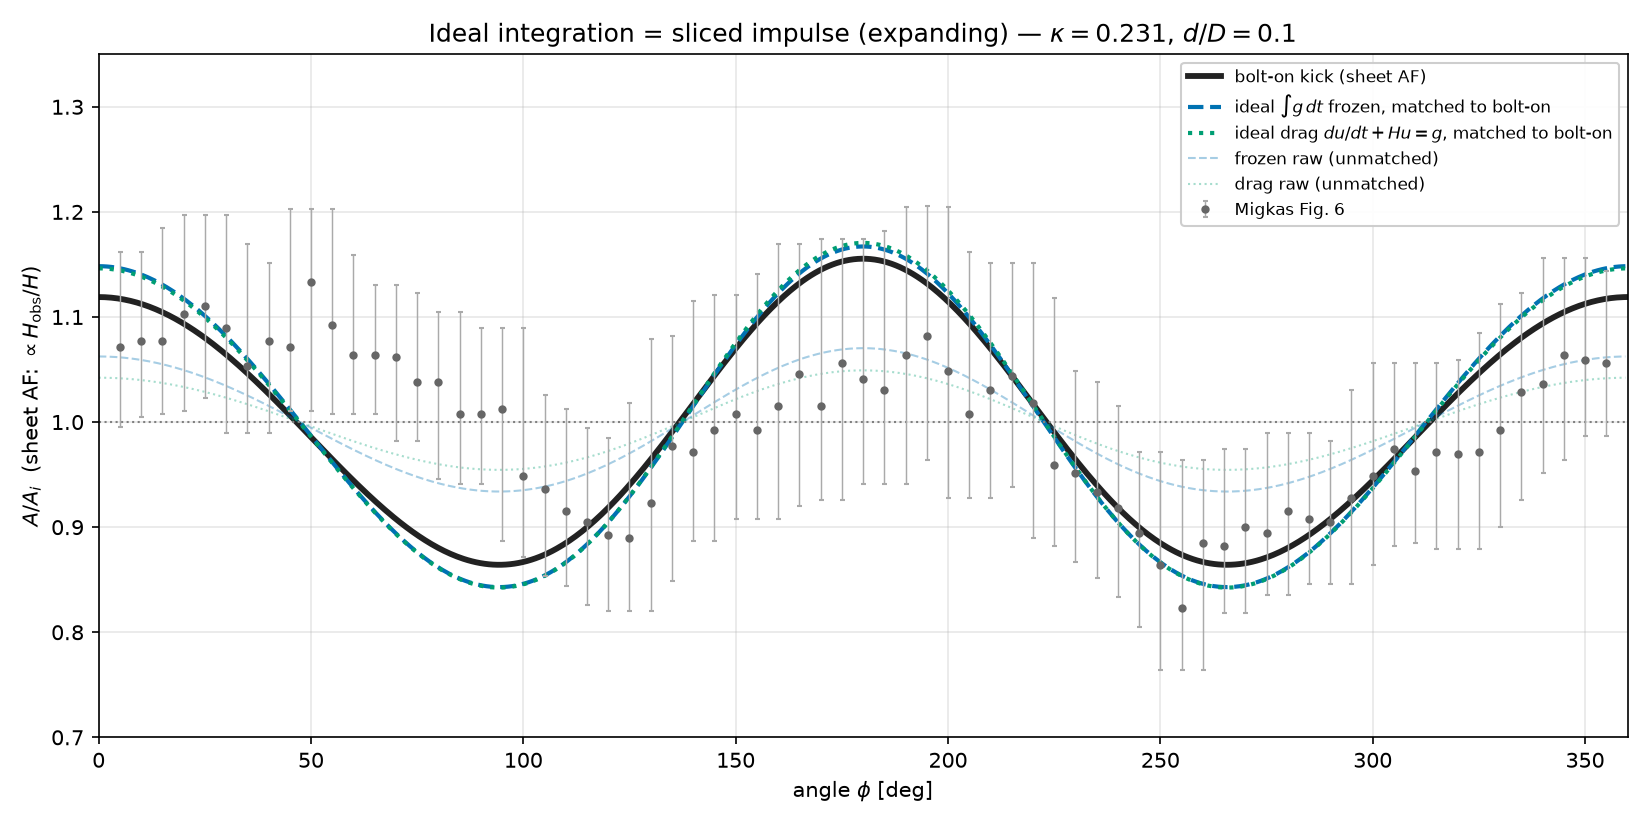
\includegraphics[width=0.88\textwidth]{A_vs_angle_ideal_integration_sheet_AF.png}
\caption{Ideal time-integrated ST+Gauss $A(\varphi)$ in the sheet AF
($A_{\mathrm{hratio}}\propto H_{\mathrm{obs}}/H$) convention, compared to
digitised Migkas Fig.~6 longitude bars. Illustrative expanding slice
($\kappa\approx0.231$, $d/D=0.1$); bolt-on versus matched ideal drag / frozen
curves coincide in angular shape. First-principles geometry only---no
Amp$\times\sin$ or $2\ell$ multiplier.}
\label{fig:idealAF}
\end{figure}

Closed forms for the circle map follow Eqs.~\eqref{eq:bolton}--\eqref{eq:Hobs}
(or the same spatial structure with $\alpha\to\alpha_{\mathrm{eff}}$). Residual
maps $\Psi=H_{\mathrm{obs}}-H$ vanish identically when $M=0$ or $\alpha=0$
(homology regression test).

%----------------------------------------------------------------------
\section{Fits: level sets, $R^2$ ladder, and residuals}
\label{sec:fits}

Correlation / affine $R^2$ is computed against digitised Migkas $A(\ell)$ along
the same chain that produced \texttt{best\_fit\_2ell\_multiplier.npz}.

\subsection{Geometry grid (first principles)}
Scanning $(M/M_0,\,d/D,\,L)$ on ideal ST+Gauss+$A_{\mathrm{hratio}}$ maps, the
top geometry without Amp$\times\sin$ rotation sits near
\begin{equation}
\frac{M}{M_0}=3,\qquad \frac{d}{D}=0.5,\qquad L\approx0.169
\quad\bigl(D/L\approx5.9\bigr),
\end{equation}
with associated $\kappa\sim\mathcal{O}(0.7)$. Ideal ST+Gauss geometry alone
yields
\begin{equation}
R^2\approx0.543
\end{equation}
against Migkas $A(\ell)$---a nontrivial longitude-pattern match, but far from
a closed case.

\begin{figure}[t]
\centering
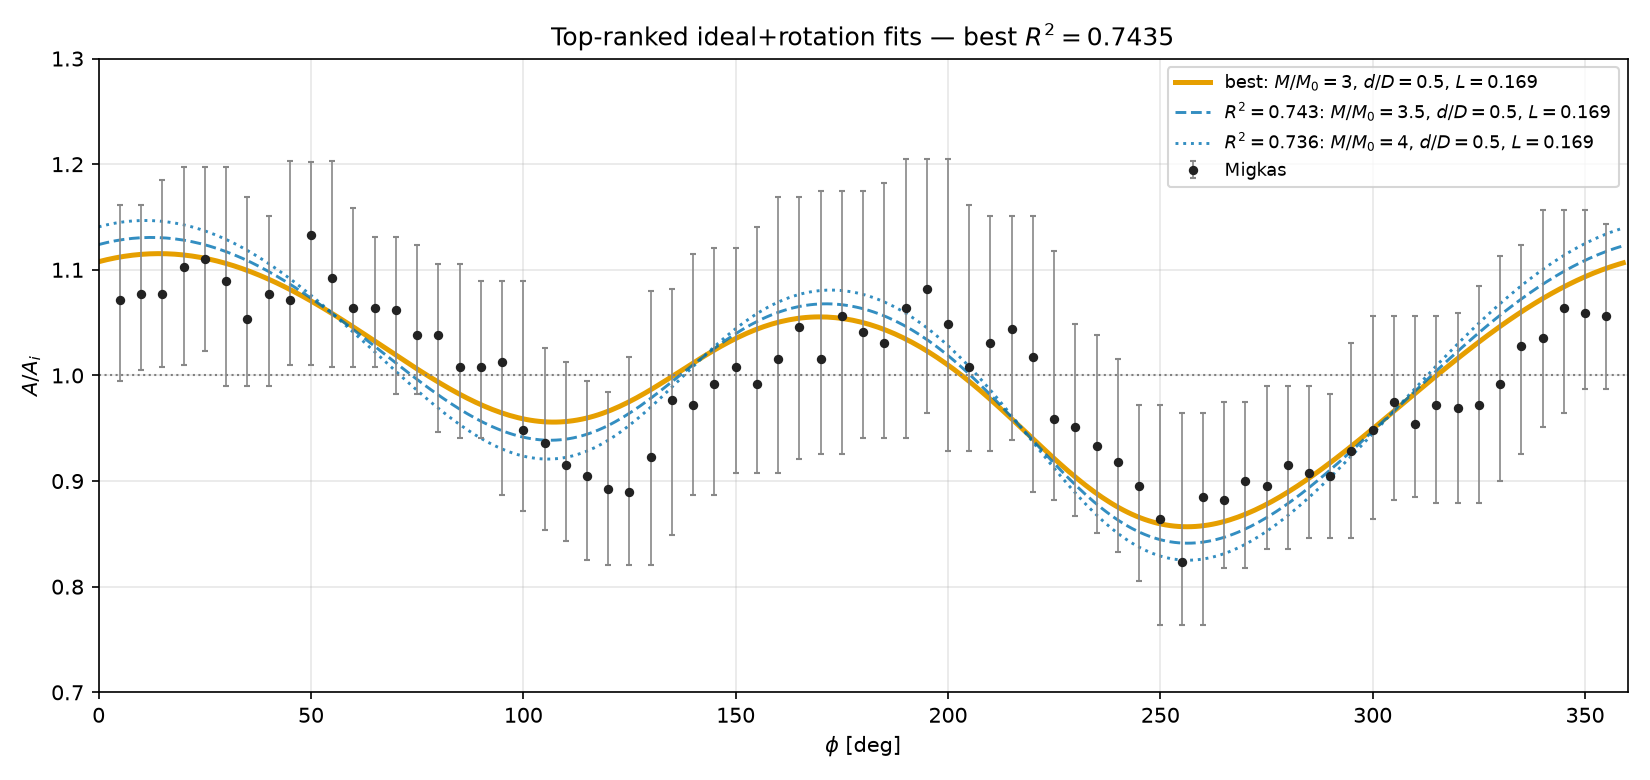
\includegraphics[width=0.88\textwidth]{ideal_rotation_3x3x5_top_curves.png}
\caption{Top geometry-grid curves from the ideal-integration
$(M/M_0,d/D,L)$ scan after Amp$\times\sin$ alignment (diagnostic). Best raw
geometry alone is $R^2\approx0.543$ ($M/M_0=3$, $d/D=0.5$, $L\approx0.169$);
with rotation the grid peak is $R^2\approx0.74$.}
\label{fig:geomgrid}
\end{figure}

\subsection{\texorpdfstring{$R^2$}{R2} ladder (honesty about knobs)}
\label{sec:ladder}

\begin{table}[t]
\centering
\caption{$R^2$ ladder versus digitised Migkas $A(\ell)$. First row is
first-principles; subsequent rows add diagnostic / phenomenological layers.}
\label{tab:ladder}
\begin{tabular}{@{}lccc@{}}
\toprule
Layer & Free knobs & $R^2$ & RMSE \\
\midrule
Ideal ST+Gauss geometry alone & geometry $(M,d/D,L)$ & $\approx0.543$ & --- \\
+ Amp$\times\sin$ phase rotation & Amp, $\phi$ & $\approx0.746$ & $0.038$ \\
+ multiplicative $2\ell$ & $\varepsilon$, $\psi$ & $\approx0.875$ & $0.029$ \\
\bottomrule
\end{tabular}
\end{table}

\paragraph{Amp$\times\sin$ rotation (diagnostic).}
Aligning the model to Galactic longitude with a sheet-style phase factor,
\begin{equation}
A_{\mathrm{rot}}(\ell)=A(\ell)+\mathrm{Amp}\,\sin(\omega\ell+\phi),
\label{eq:ampsin}
\end{equation}
with best Amp / $\phi$ level
\begin{equation}
\mathrm{Amp}=-0.06,\qquad \phi\approx0.20\,\mathrm{rad}
\quad(R^2\approx0.746).
\end{equation}
(The same chain's residual-$2\ell$ file used $\phi_1\approx0.30$ with Amp$=-0.06$
as a nearby local maximum; both sit on the Amp$=-0.06$ ridge.)

\begin{figure}[t]
\centering
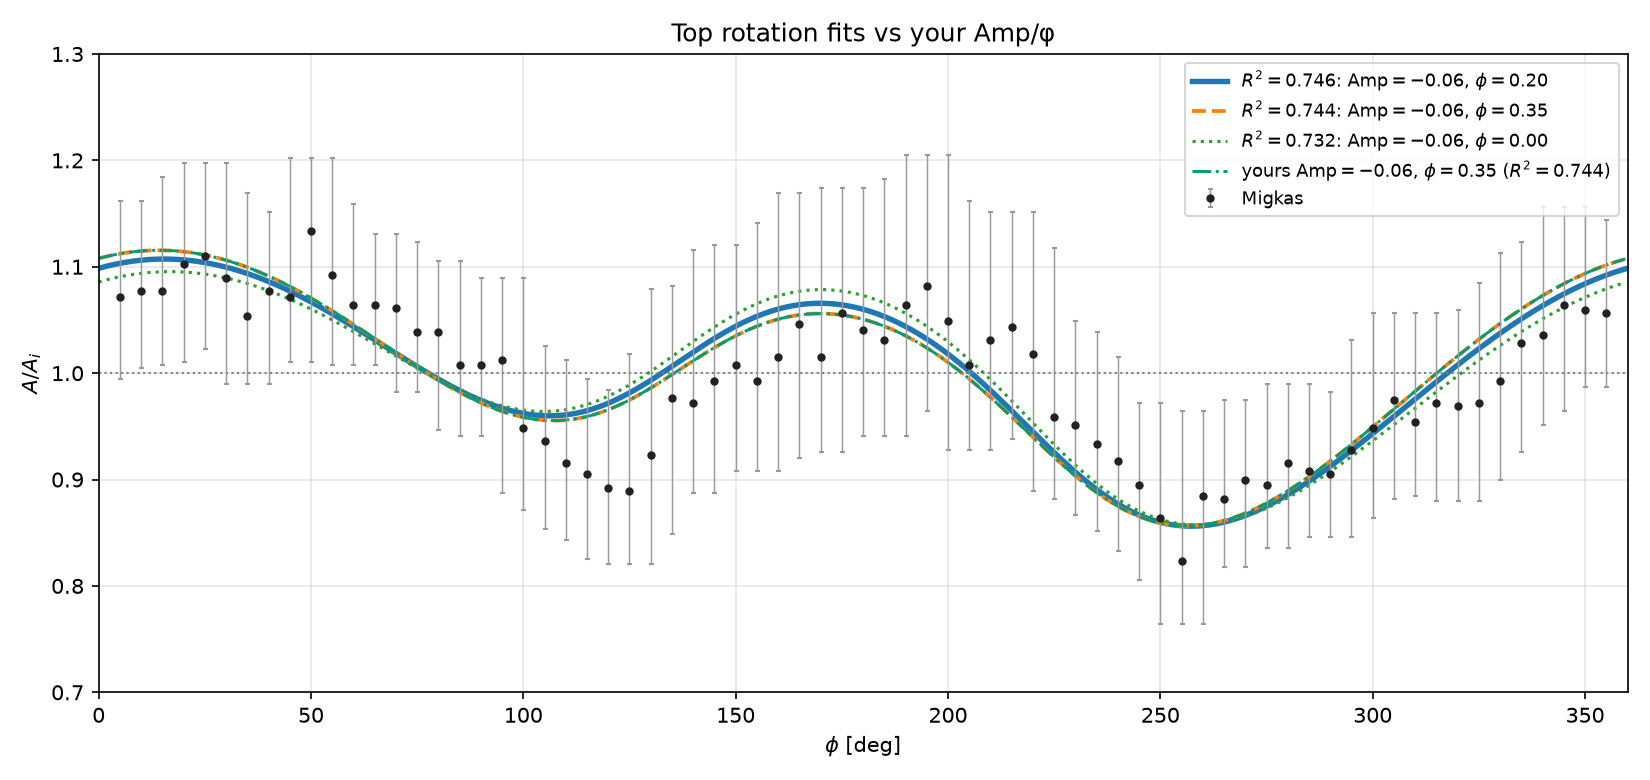
\includegraphics[width=0.88\textwidth]{rotation_Amp_phi_top_curves.png}
\caption{Amp$\times\sin$ scan: top curves in $(\mathrm{Amp},\phi)$. Diagnostic
layer only---phase can encode non-radial observer velocity or sky-axis
misalignment, not a first-principles prediction.}
\label{fig:ampphi}
\end{figure}

\begin{figure}[t]
\centering
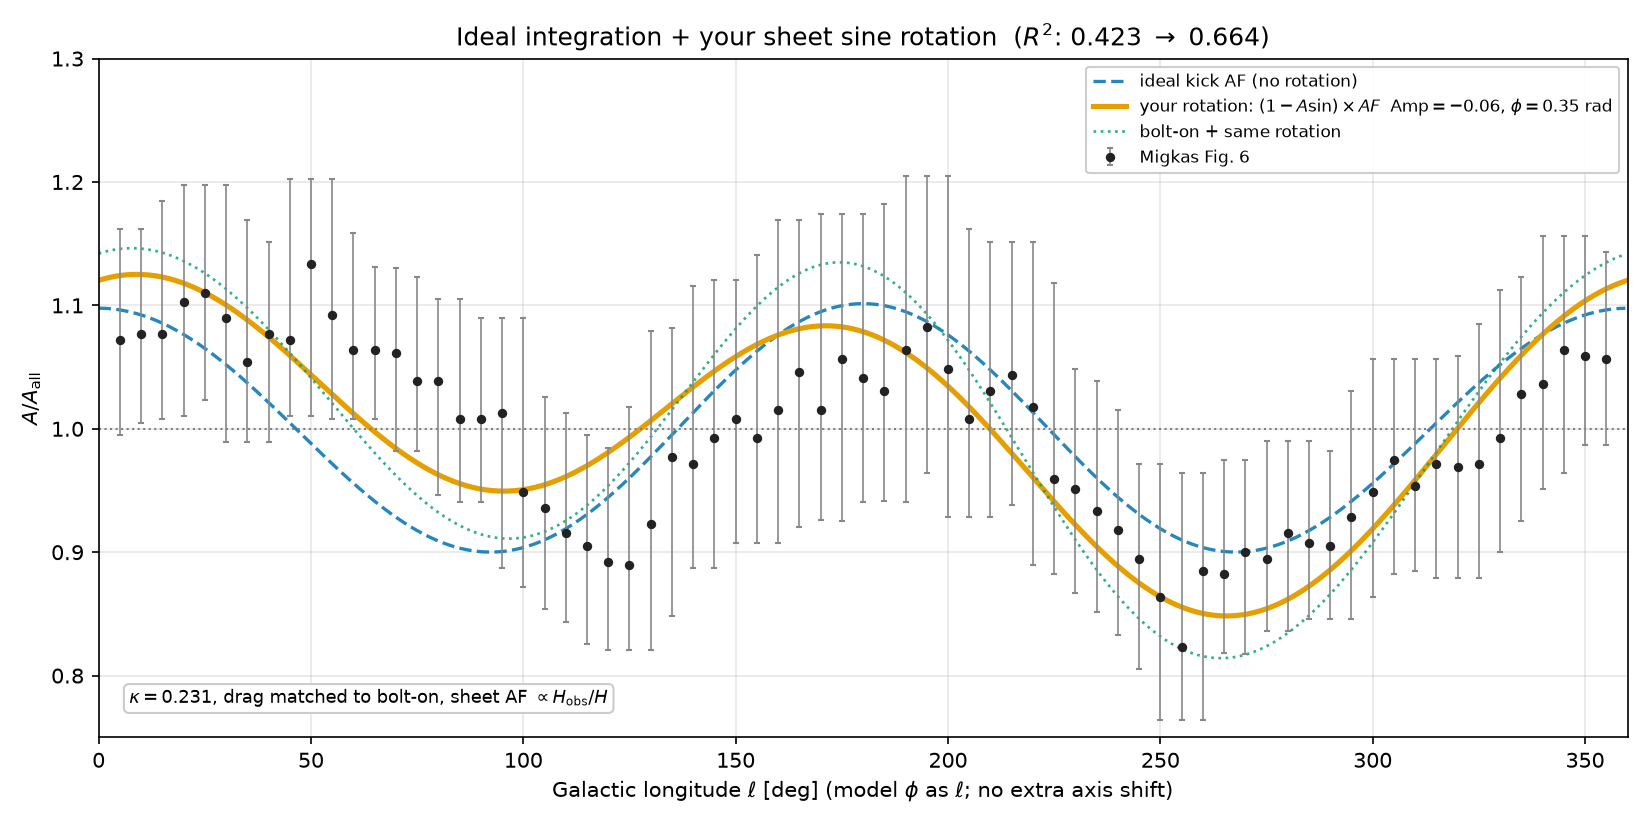
\includegraphics[width=0.88\textwidth]{A_vs_angle_ideal_plus_chris_rotation.png}
\caption{Sheet-style ideal ST+Gauss $A_{\mathrm{hratio}}$ (AF) after
Amp$\times\sin$ rotation (Amp$=-0.06$, $\phi\approx0.35\,\mathrm{rad}$ on
this illustrative $\kappa{=}0.231$, $d/D{=}0.1$ slice) overlaid on Migkas
bars. Geometry is first-principles; the rotation is diagnostic. This panel is
\emph{not} the Table~\ref{tab:ladder} peak ($R^2\approx0.746$ at
$\phi\approx0.20\,\mathrm{rad}$ on the best geometry).}
\label{fig:rotated}
\end{figure}

\paragraph{Multiplicative $2\ell$ residual (phenomenological).}
Leftover quadrupole structure after Amp$\times\sin$ is absorbed by
\begin{equation}
A\;\leftarrow\;\bigl(1+\varepsilon\sin(2\ell+\psi)\bigr)\,A,
\label{eq:2ell}
\end{equation}
with best values from the project's NPZ chain
\begin{equation}
\varepsilon\approx-0.043,\qquad \psi\approx176^\circ,
\end{equation}
raising
\begin{equation}
R^2:\;0.746\rightarrow0.875,\qquad
\mathrm{RMSE}:\;0.038\rightarrow0.029.
\end{equation}

\begin{figure}[t]
\centering
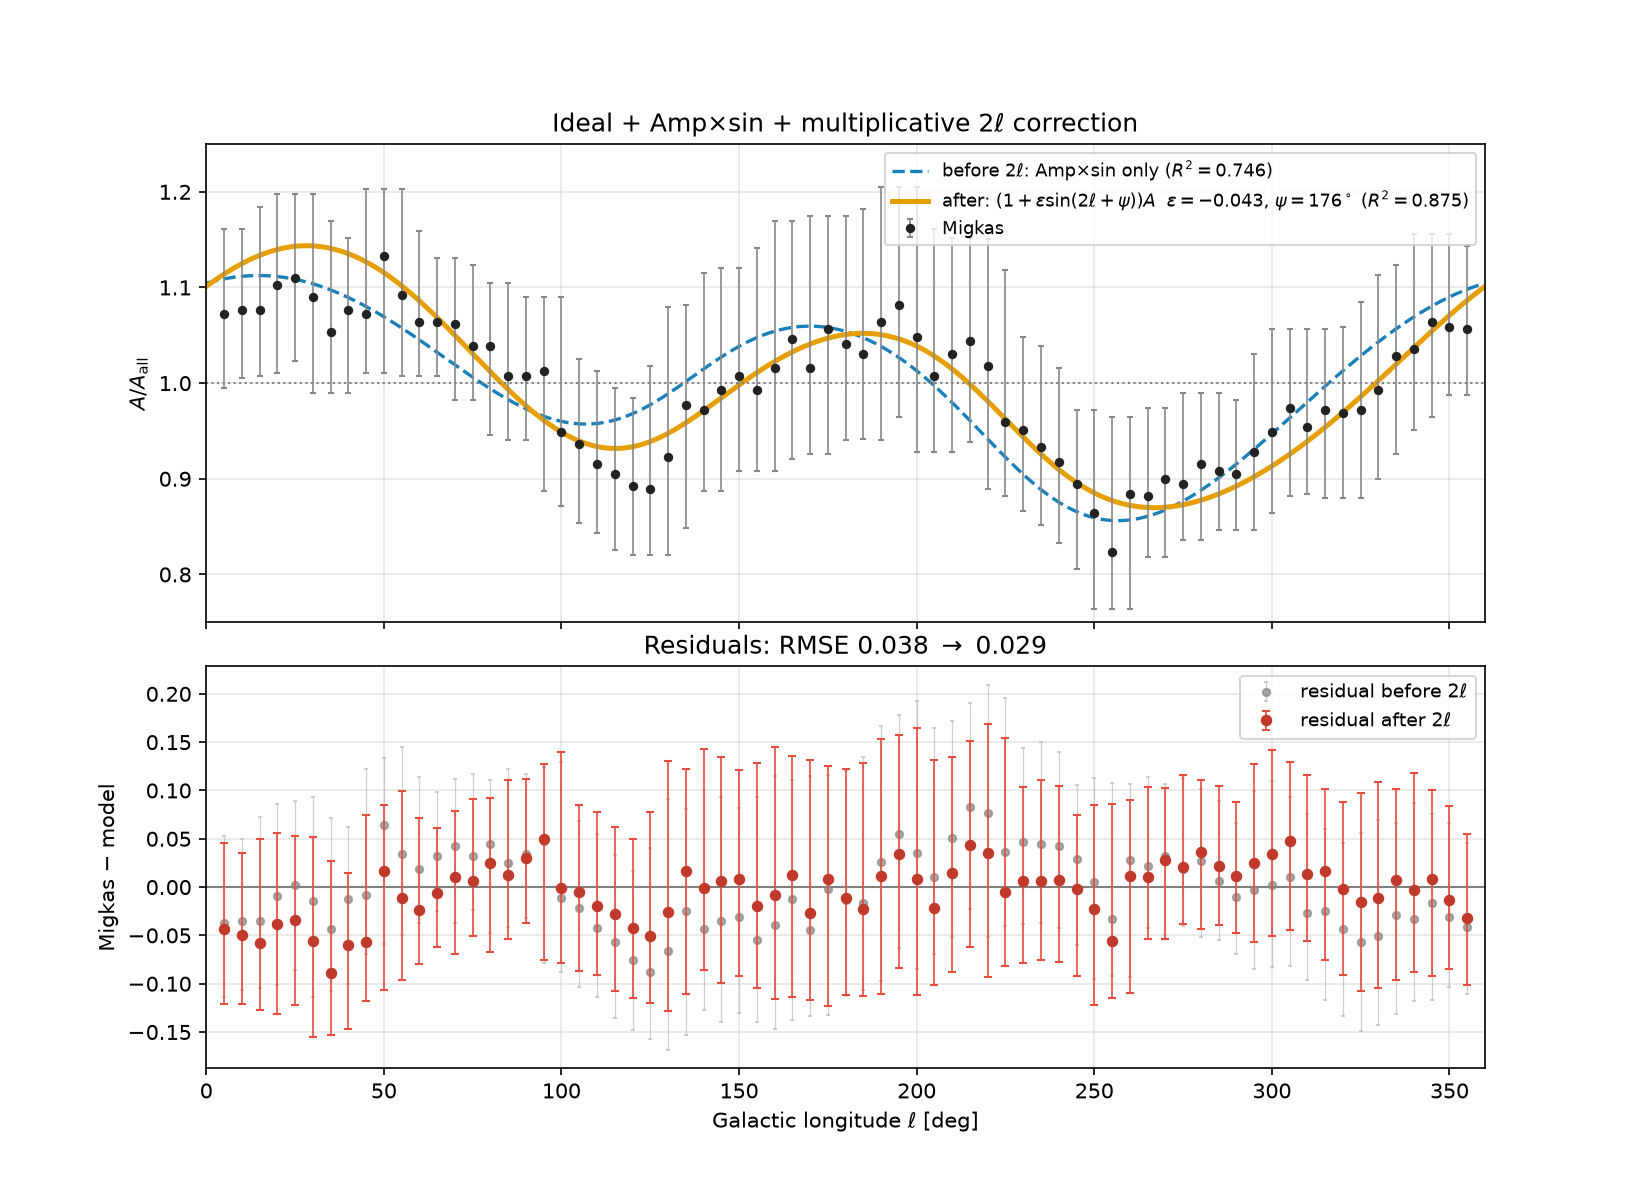
\includegraphics[width=0.92\textwidth]{best_fit_with_2ell_multiplier.png}
\caption{\textbf{Key fit figure.} Best ST+Gauss + Amp$\times\sin$ model with
multiplicative $2\ell$ correction versus Migkas $A(\ell)$. The geometric
backbone is first-principles; Amp$\times\sin$ and $2\ell$ are diagnostic /
phenomenological layers. Part of the high $R^2$ is knobs---stated explicitly.}
\label{fig:best2ell}
\end{figure}

\textbf{Honesty clause:} Amp$\times\sin$ and the $2\ell$ multiplier are
\emph{not} derived from ST+Gauss alone. They are diagnostic layers (phase from
possible non-radial observer velocity or axis misalignment; $2\ell$ as leftover
quadrupole). The first-principles claim is the geometry that already achieves
$R^2\approx0.54$ before knobs. Reporting $R^2\approx0.88$ without that
decomposition would be cheerleading.

%----------------------------------------------------------------------
\section{Physical reading of Amp$\times\sin$, $2\ell$, and nesting dolls}
\label{sec:reading}

\paragraph{Amp$\times\sin$.}
A pure radial peculiar field $\vec{u}\propto-\hat{r}$ about the CoE produces a
fixed angular template once $\hat{D}$ is chosen. An additional non-radial
observer velocity (or a misidentified preferred axis on the sky) mixes a
sinusoidal longitude modulation into the observed $A(\ell)$. The Amp$\times\sin$
layer is the minimal phenomenological proxy for that mixing. It should not be
read as evidence that ST+Gauss ``predicts'' Amp$=-0.06$.

\paragraph{$2\ell$ multiplier.}
At $d\ll D$ (CoE beyond the horizon, clusters at hundreds of Mpc), the linear
tidal map of a spherical Gauss field is dominated by a \emph{quadrupole}
$P_2(\mu)$, not a pure dipole~\citep{Heinesen2020}. Migkas Fig.~6 is a
one-dimensional longitude projection; footprint leakage can project quadrupole
power into an apparent dipole-like strip pattern. The multiplicative $2\ell$
term absorbs residual quadrupole after the leading geometric template and
Amp$\times\sin$ are fixed. Again: diagnostic, not first principles.

\begin{figure}[t]
\centering
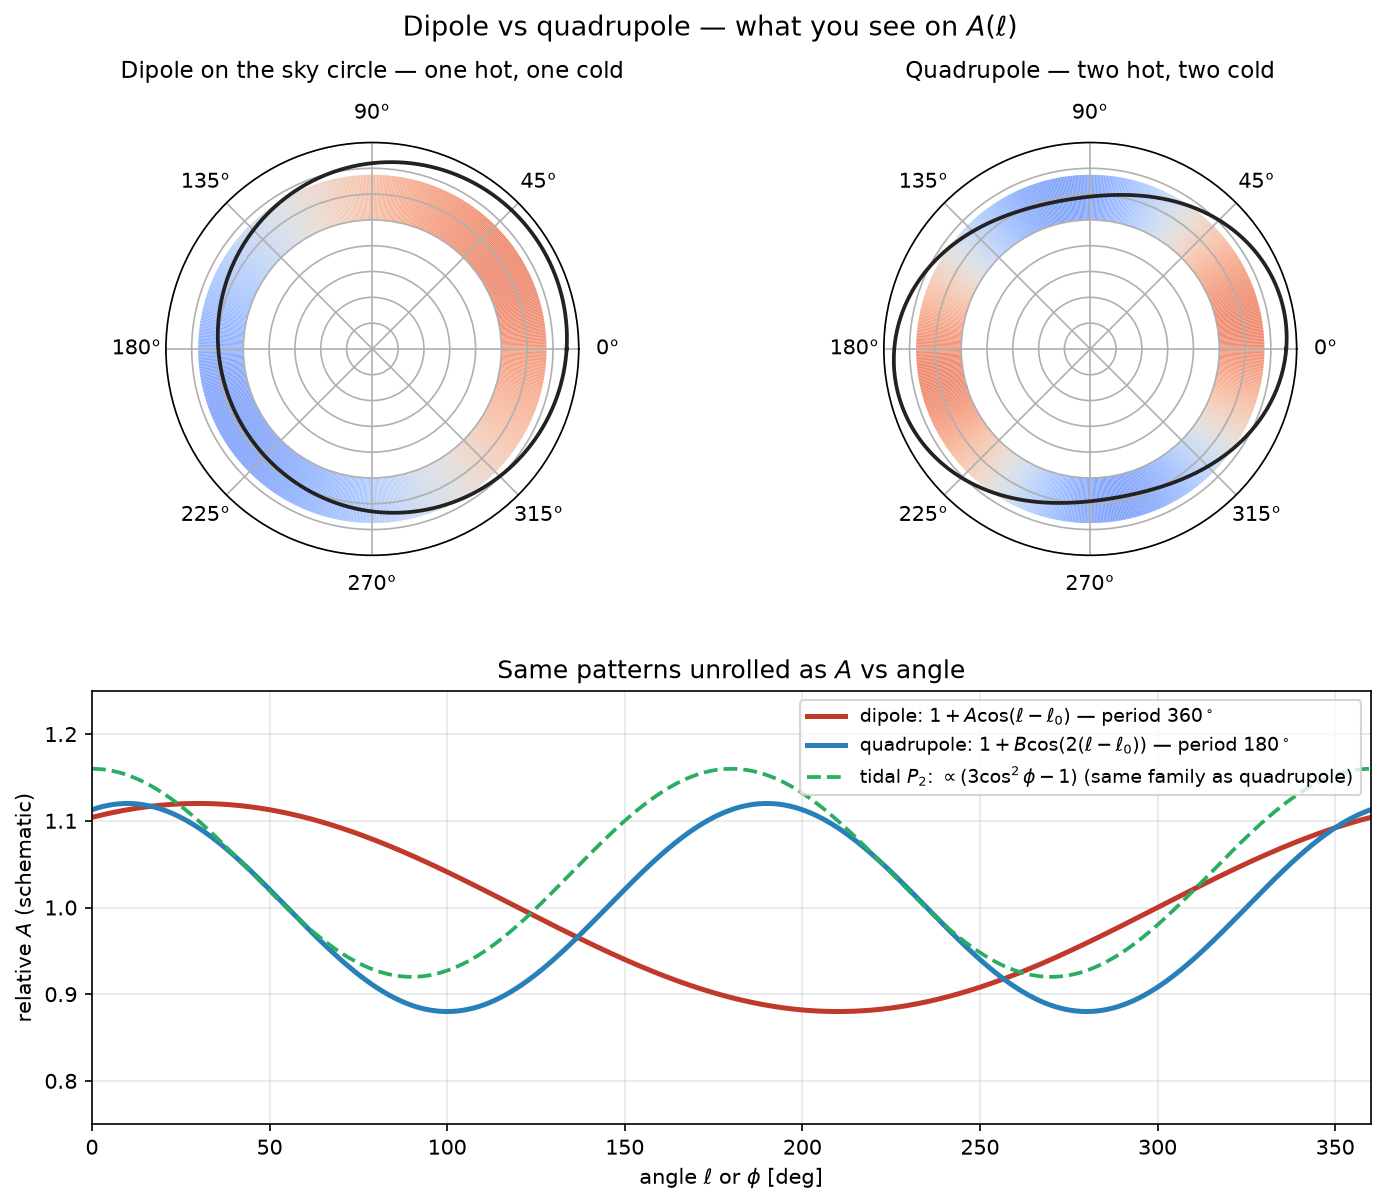
\includegraphics[width=0.88\textwidth]{dipole_vs_quadrupole_examples.png}
\caption{Schematic dipole versus quadrupole patterns on the ST+Gauss sky
(bottom: unrolled $A$ versus angle). At small $d/D$ the leading Gauss tidal
anisotropy is quadrupole-like ($P_2$); Migkas longitude strips mix multipoles.
Legend coefficients $A$/$B$ here are schematic multipole amplitudes, not
Migkas strip normalizations.}
\label{fig:dipquad}
\end{figure}

\paragraph{Nesting dolls (speculation).}
Optional outer off-center masses---``nesting dolls'' of additional centers---could
source leftover multipoles beyond $2\ell$. This is marked as
\textbf{speculation}: it is not required by the $R^2$ ladder, is not constrained
by the present Newtonian pass, and must not be sold as part of the ST+Gauss
core.

\begin{figure}[t]
\centering
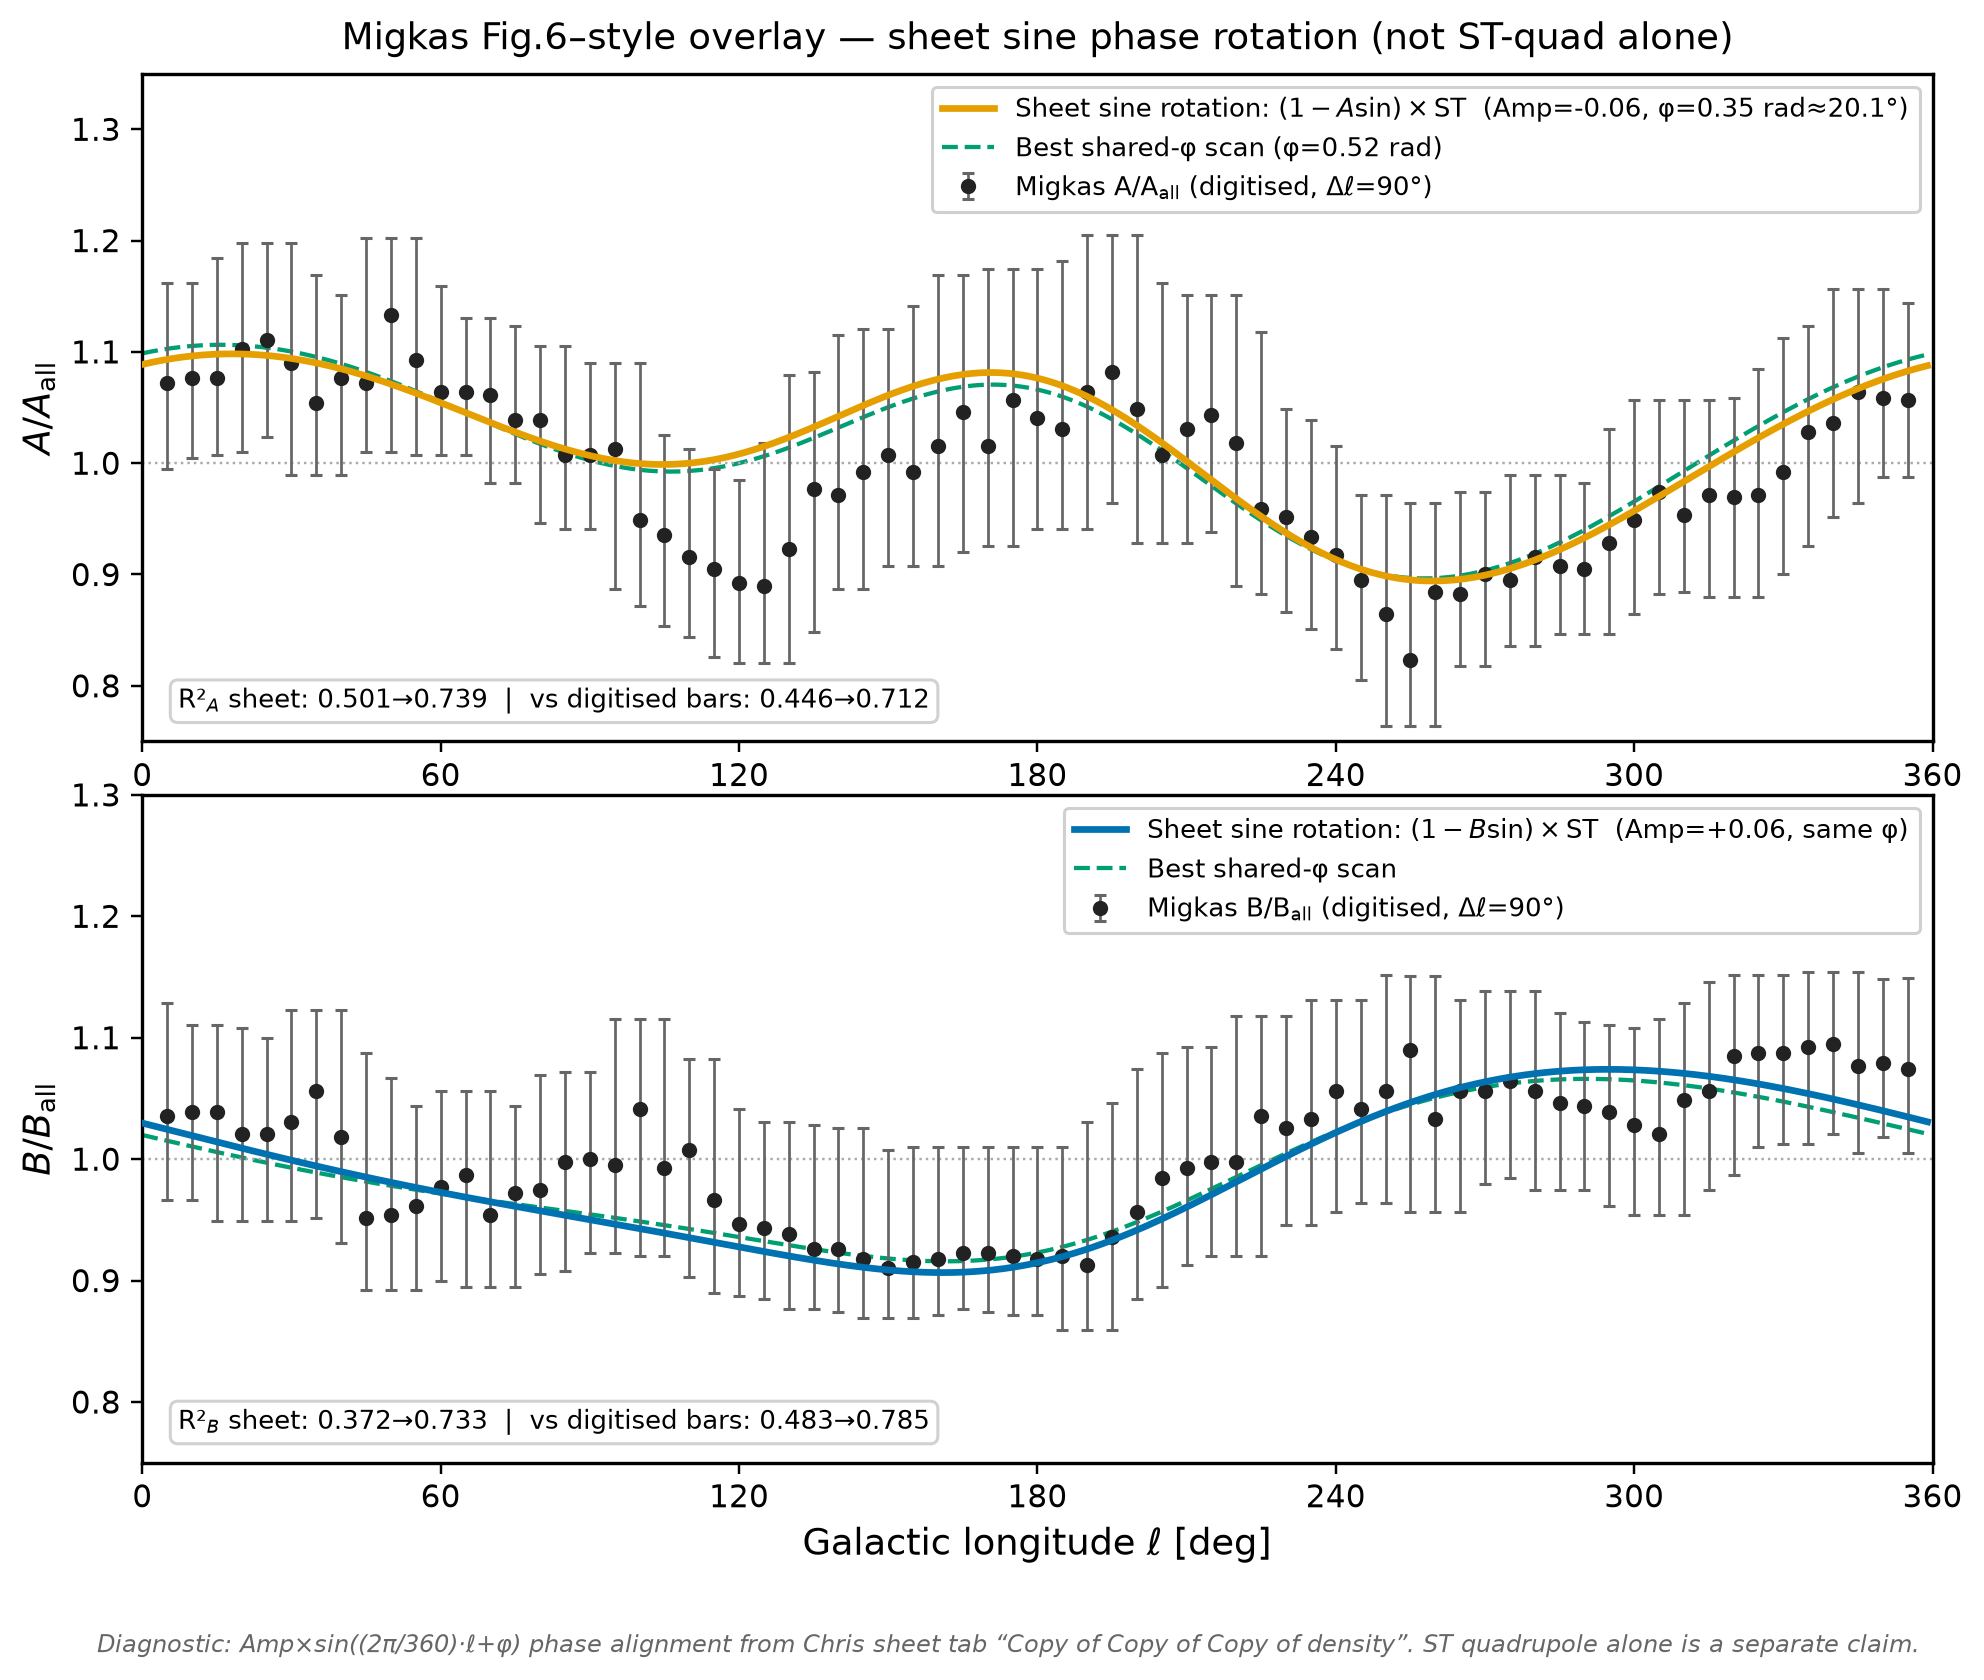
\includegraphics[width=0.88\textwidth]{migkas_bars_rotation_overlay.png}
\caption{Migkas longitude bars with Amp$\times\sin$ overlays.
\textbf{Top:} Migkas~$A$ (the quantity used in the $R^2$ ladder).
\textbf{Bottom:} Migkas~$B$ (ancillary strip normalization; \emph{not} used
in Table~\ref{tab:ladder}). Phase values on this panel sit on the Amp$=-0.06$
ridge near $\phi\approx0.35\,\mathrm{rad}$; the ladder peak quoted in the text
is Amp$=-0.06$, $\phi\approx0.20\,\mathrm{rad}$. Diagnostic methods figure.}
\label{fig:migkasoverlay}
\end{figure}

%----------------------------------------------------------------------
\section{Related work}
\label{sec:related}

\textbf{Fennelly~\citep{Fennelly1977}} fitted reported Hubble anisotropy to a
tilted self-similar cosmology with a Gaussian density inhomogeneity, placing
us $\sim120\,\mathrm{Mpc}$ off-center. Conceptual cousin (off-center observer,
CMB-compatibility concern); not ST+Gauss, not Migkas $A(\ell)$.

\textbf{Debney~\citep{Debney1977} / Pathria~\citep{Pathria1972} /
Khakshournia~\citep{Khakshournia2014}.}
``Universe as a black hole'' / beyond-horizon matching language. Khakshournia
shows Pathria-style null matching is not smooth (surface pressure on a null
shell)---a warning against naive horizon identification.

\textbf{Bertschinger~\citep{Bertschinger1983}.}
Closest classical ST-in-cosmology dynamics: Sedov-like blast morphing into a
thin dense shell in EdS. Supplies blast DNA, not off-center Migkas matching.

\textbf{Smoller \& Temple~\citep{SmollerTemple1998,SmollerTemple2002}.}
Exact FRW--TOV shock matching, including a Big Bang as a localized explosion
inside an asymptotically flat Schwarzschild black hole with shock beyond a
Hubble length. Closest GR cousin for beyond-horizon CoE ontology; continuum
shock matching rather than time-integrated Gauss $g$.

\textbf{Alnes \& Amarzguioui~\citep{Alnes2006}; Kodama et~al.~\citep{Kodama2010};
Blomqvist \& M{\"o}rtsell~\citep{Blomqvist2010}.}
Off-center LTB voids: CMB dipole forces the observer within
$\sim15$--$16\,\mathrm{Mpc}$ of the center; SNIa alone are much weaker.
Transfers the CMB-adversary toolkit to any spherical CoE.

\textbf{Heinesen~\citep{Heinesen2020}.}
Model-independent multipole decomposition of the anisotropic $d_L$ Hubble law
(9 / 25 / 61 dof at $\mathcal{O}(z)$ / $\mathcal{O}(z^2)$ / $\mathcal{O}(z^3)$).
Language layer for forecasting ST+Gauss $d_L(\hat{n},z)$ without committing to
FLRW.

\textbf{Saadeh et~al.~\citep{Saadeh2016}.}
Planck T+P Bianchi VIIh analysis: anisotropic expansion odds
$\sim1.2\times10^5:1$ against; $(\sigma_V/H)_0<4.7\times10^{-11}$ (95\%).
Constrains \emph{homogeneous} anisotropy; does not identically kill an
inhomogeneous spherical CoE, but forbids reading Migkas as global shear.

\textbf{Migkas et~al.~\citep{Migkas2020}.}
Primary empirical target: Fig.~6 $A$ versus Galactic longitude.

%----------------------------------------------------------------------
\section{Discussion: what a good fit does and does not prove}
\label{sec:discussion}

\subsection{\texorpdfstring{What $R^2\approx0.54$--$0.88$ means}{What R2 approx 0.54--0.88 means}}
A geometric ST+Gauss off-center template that correlates with Migkas longitude
at $R^2\approx0.54$ before knobs is interesting: it is not noise-shaped
cherry-picking of a free dipole. Raising $R^2$ to $\sim0.75$--$0.88$ with
Amp$\times\sin$ and $2\ell$ shows that residual phase and quadrupole structure
are absorbable---but those layers are knobs. A good fit does \emph{not} prove a real CoE, does not prove that Migkas is
cosmological rather than systematic, and does not waive CMB constraints.

\subsection{CMB adversary}
Planck isotropy~\citep{Planck2018VII} remains the ceiling. In spherical
inhomogeneous models, an off-center observer induces a CMB dipole that forces
offsets $\lesssim 15\,\mathrm{Mpc}$ in standard void constructions
\citep{Alnes2006,Kodama2010}. A CoE \emph{beyond the horizon} is a stronger
claim than a Gpc void with us near center: it requires a mechanism by which last
scattering looks nearly isotropic while $z\lesssim0.3$ clusters show
$\mathcal{O}(10\%)$ effects. Without that mechanism, the CMB wins. SNIa alone
do not tighten the bound~\citep{Blomqvist2010}.

Saadeh et~al.~\citep{Saadeh2016} nearly exclude Bianchi shear. That is
\textbf{not} the same as excluding an inhomogeneous CoE, but it forbids
conflating ``anisotropic $H_{\mathrm{obs}}$ about us'' with ``globally
anisotropic expansion.''

\subsection{Falsifiers}
The program is falsifiable, among other ways, by:
\begin{enumerate}[leftmargin=*,itemsep=2pt]
\item A demonstrated X-ray / selection systematic that erases Migkas Fig.~6
  without a cosmological $A(\ell)$.
\item A CMB-compatible construction that cannot simultaneously host
  $\mathcal{O}(10\%)$ late-time $A(\ell)$ from a beyond-horizon CoE.
\item Homology regression failure in the forward model ($M=0$ still anisotropic).
\item Expand/collapse morphology that cannot be reconciled with the observed
  trough/peak placement once $A_{\mathrm{hratio}}$ is fixed.
\item Multipole structure (full-sky $C_\ell$) incompatible with cone-scan /
  longitude-strip data once footprint is modeled honestly.
\end{enumerate}

\subsection{Open problems}
No GR metric, no light-travel-time $H_{\mathrm{obs}}$, no self-consistent
ST+gravity similarity solution, and no beyond-horizon matching that survives
Khakshournia-type junction scrutiny~\citep{Khakshournia2014} are provided here.
$\alpha_{\mathrm{eff}}$ and $\kappa$ remain order-unity parameters, not
microphysically fixed.

%----------------------------------------------------------------------
\section{Conclusions}
\label{sec:concl}

We synthesize the Newtonian ST+CoE program as follows:
\begin{itemize}[leftmargin=*,itemsep=2pt]
\item Real CoE beyond the horizon; off-center observer in homologous ST
  expansion or collapse.
\item Gauss gravity with decreasing $\rho(r)$ and enclosed mass toward the CoE;
  $\kappa\sim\mathcal{O}(0.1$--$1)$ versus $M_{\mathrm{crit}}$ is intended as
  natural, not extreme.
\item Ideal time-integrated gravity is preferred over bolt-on
  $u\sim\alpha g/H$: integration rescales amplitude only
  ($\alpha_{\mathrm{eff}}\sim2/3$ with Hubble drag); expand versus collapse
  flips the $A(\varphi)$ shape.
\item Primary Migkas comparison uses
  $A_{\mathrm{hratio}}\propto H_{\mathrm{obs}}/H$.
\item $R^2$ ladder: $0.543$ (geometry) $\to$ $0.746$ (Amp$\times\sin$) $\to$
  $0.875$ ($2\ell$), with Amp$=-0.06$, $\phi\approx0.20\,\mathrm{rad}$,
  $\varepsilon\approx-0.043$, $\psi\approx176^\circ$, and top geometry
  $M/M_0=3$, $d/D=0.5$, $L\approx0.169$.
\item Amp$\times\sin$ and $2\ell$ are diagnostic / phenomenological; nesting
  dolls are speculative.
\item The CMB remains the adversary (Alnes/Kodama $\sim15\,\mathrm{Mpc}$);
  Saadeh Bianchi bounds constrain homogeneous shear, not an inhomogeneous CoE
  identically. This draft does not claim to have falsified the cosmological
  principle.
\end{itemize}

%----------------------------------------------------------------------
\section*{Acknowledgments}
\label{sec:ack}

Conversations with Wolfgang Rindler and Luke Ackerman---especially night
conversations after general mechanics and relativity courses---shaped the
genesis of this centered-universe program and are gratefully acknowledged.
Errors, overclaims, and remaining tensions with the CMB are the author's alone.

%----------------------------------------------------------------------
\begin{thebibliography}{99}

\bibitem[Alnes and Amarzguioui(2006)]{Alnes2006}
H.~Alnes and M.~Amarzguioui,
CMB anisotropies seen by an off-center observer in a spherically symmetric
inhomogeneous universe,
Phys.\ Rev.\ D \textbf{74}, 103520 (2006), arXiv:astro-ph/0607334.

\bibitem[Bertschinger(1983)]{Bertschinger1983}
E.~Bertschinger,
Self-similar secondary infall and accretion in an Einstein--de Sitter universe,
Astrophys.\ J.\ \textbf{268}, 17 (1983).

\bibitem[Blomqvist and M{\"o}rtsell(2010)]{Blomqvist2010}
M.~Blomqvist and E.~M{\"o}rtsell,
Supernovae as seen by off-center observers in a local void,
JCAP \textbf{05}, 006 (2010), arXiv:0909.4723.

\bibitem[Debney(1977)]{Debney1977}
G.~Debney,
Techniques of global analysis: a cosmological black hole?,
NASA TM X-73378 (1977).

\bibitem[Fennelly(1977)]{Fennelly1977}
A.~J.~Fennelly,
Mon.\ Not.\ R.\ Astron.\ Soc.\ \textbf{181}, 121 (1977).

\bibitem[Heinesen(2021)]{Heinesen2020}
A.~Heinesen,
Multipole decomposition of the general luminosity distance Hubble law,
JCAP \textbf{05}, 008 (2021), arXiv:2010.06534.

\bibitem[Khakshournia(2014)]{Khakshournia2014}
S.~Khakshournia,
A note on Pathria's model of the universe as a black hole,
arXiv:1412.0105 (2014).

\bibitem[Kodama et~al.(2010)]{Kodama2010}
H.~Kodama, K.~Saito, and A.~Ishibashi,
Analytic formulae for CMB anisotropy for off-center observers in spherical
symmetry, arXiv:1004.3089 (2010).

\bibitem[Migkas et~al.(2020)]{Migkas2020}
K.~Migkas et~al.,
Probing cosmic isotropy with a new X-ray galaxy cluster sample through the
$L_X$--$T$ scaling relation,
Astron.\ Astrophys.\ \textbf{636}, A15 (2020), arXiv:2004.03305.

\bibitem[Pathria(1972)]{Pathria1972}
R.~K.~Pathria,
The Universe as a black hole,
Nature \textbf{240}, 298 (1972).

\bibitem[Planck Collaboration(2020)]{Planck2018VII}
Planck Collaboration,
Planck 2018 results. VII. Isotropy and statistics of the CMB,
Astron.\ Astrophys.\ \textbf{641}, A7 (2020).

\bibitem[Saadeh et~al.(2016)]{Saadeh2016}
D.~Saadeh, S.~M.~Feeney, A.~Pontzen, H.~V.~Peiris, and J.~D.~McEwen,
How isotropic is the Universe?,
Phys.\ Rev.\ Lett.\ \textbf{117}, 131302 (2016), arXiv:1605.07178.

\bibitem[Smoller and Temple(1998)]{SmollerTemple1998}
J.~Smoller and B.~Temple,
Cosmology with a shock-wave,
Commun.\ Math.\ Phys.\ \textbf{210}, 275 (1998).

\bibitem[Smoller and Temple(2003)]{SmollerTemple2002}
J.~Smoller and B.~Temple,
Shock-wave cosmology inside a black hole,
Proc.\ Natl.\ Acad.\ Sci.\ USA \textbf{100}, 11216 (2003), arXiv:astro-ph/0210105.

\end{thebibliography}

\end{document}
